\chapter{Verwendete Technologien}\label{cha:theoretical-background}
\section{Entität Framework}
(Referenz Wikipedia)
Dabei handelt es sich um ein Framework zur Erstellung von objektrelationalen Abbildungen (ORM – object relational mapping) auf .NET-Objektstrukturen. Dieses Framework wurde von Microsoft entwickelt.
\newline
Zum Modellieren einer Datenbank gibt es zwei Ansätze, nämlich Code First und Model First. Zur Erstellung der verwendeten Datenbank wurde die erste Methode gewählt, nämlich Code First (Entity Framework 4.6.1). Dazu werden die Klassen im Programm zuerst definiert und darauf basierend wird vom DbContext die Datenbank erzeugt. Als Alternative bietet sich Model First an, wobei zuerst die Entity-Klassen mit Hilfe eines grafischen Tools modelliert werden und danach vom Grafischen in Code-Klassen und Datenbanktabellen umgewandelt werden.
Der wohl wichtigste Bestandteil des Entity Frameworks ist der ApplicationDbContext (Name selbst vergeben). Dieser implementiert das Interface DbContext und enthält DbSets aller Datenbankklassen. Er stellt die Verbindung zur Datenbank über den Connectionstring her, der im Konstruktor gesetzt wird.  
\newline Ein DbSet ist eine Klasse, die die entsprechenden Methoden für Entitätstypen anbietet.
\subsection{Linq}
(Referenz Wikipedia)
Linq steht abgekürzt für Language Integrated Query und ermöglicht den Zugriff auf Daten aus einem Programm. Dabei kann der Benutzer auf lokale Listen im Programm zugreifen, auf Daten aus der Datenbank, auf XML-Inhalte und vieles mehr. Im Falle dieser Arbeit wird aber nur Linq to Objects und Linq to Entities verwendet. Standardmethoden wie Where oder Select, die in SQL genauso benutzt werden, werden sehr gerne verwendet. 
\newline Linq hat die Eigenschaft, dass die gegebenen Ausdrücke nicht bei ihrer Definition ausgeführt werden, sonder erst wenn der Wert tatsächlich gebraucht wird. Das hat zum Vorteil, dass Abfragen öfters verwendet werden können. Falls der Benutzer das nicht möchte, muss die Ergebnismenge sofort in einen anderen Datentyp  umgewandelt werden, was den häufigere Anwendungsfall beschreibt. Ein Beispiel wäre nach der Query ein .ToList() anzuhängen. 
\newline Mit der nachfolgenden Codezeile werden beispielsweise alle Kontaktlinsenaufträge gewählt, die schon bezahlt wurden.
\begin{lstlisting}
List<Order> paidContactLenses = this.ContactLenses.Where(c => c.PaymentState == "Bezahlt").ToList();
\end{lstlisting}
Ein anderes Beispiel wäre alle Kunden zu zählen, deren Vorname mit 'E' beginnt:
\begin{lstlisting}
int customersStartingFirstNameWithE = this.Customers.Count(c => c.FirstName.StartsWith("E"));
\end{lstlisting}
\section{UnitOfWork Pattern}
(Referenz CodeProject)
Das UnitOfWork Pattern ist ein Weg der Projektarchitektur für Datenbankanwendungen. Diese verwaltet Transaktionen, führt Updates geregelt durch und schafft damit Concurrency-Probleme aus der Welt. Dadurch arbeitet man im Code nicht direkt mit der Datenbank sondern mit der UnitOfWork, welche eine lokale Kopie von allen Daten beinhaltet.
Um das UnitOfWork-Pattern zu implementieren, benötigt man folgende Klassen:
\begin{itemize}
\item EntityObject: Dies ist eine Klasse, von der später alle Entitäten ableiten. Sie gibt den Entitäten eine Id und einen Timestamp, um später Concurrency-Probleme zu lösen.
\item IGenericRepository: Ein Interface, welches die Standardmethoden wie Get, Insert oder Delete vorschreibt.
\item IUnitOfWork: Ein Interface, welches die Definition für alle IGenericRepositories, die Save-Methode sowie andere Methodenköpfe, die später selbst implementiert werden enthält.
\item GenericRepository: Eine Klasse, die für jede Entität erstellt wird und die vom IGenericRepository ableitet. Sie enthält den Context sowie das DbSet der gewünschten Entität. Zusätzlich implementiert sie alle Standardmethoden (Get, GetById, Insert, Update, Delete, Count...).
\item UnitOfWork: Eine Klasse, die von IUnitOfWork ableitet und alle Methoden implementiert. Mit dieser Klasse wird später im Programm auch gearbeitet. 
\end{itemize}
Zum Beispiel wird mit diesem Befehl ein Kunde mittels der Id gefunden:
\begin{lstlisting}
Customer c = this.Uow.CustomerRepository.GetById(id);
\end{lstlisting}
Es wird also zuerst auf die UnitOfWork zugegriffen und von dort aus auf das spezielle Repository. CustomerRepository ist vom Typ GenericRepository \textless Customer  \textgreater und damit kann man auf die Standardmethoden (hier GetById) zugreifen.
\newline
Ein anderes Beispiel wäre das Einfügen eines neuen Datensatzes in die Datenbank. Dazu muss unbedingt die Save-Methode danach aufgerufen werden, denn sonst werden die Änderungen nicht in die Datenbank übertragen.
\begin{lstlisting}
this.Uow.CustomerRepository.Insert(this.Customer);
this.Uow.Save();
\end{lstlisting}
\section{Wpf}
(Referenz It-Visions)
Wpf (Windows Presentation Foundation) ist eine von Microsoft entwickelte Klassenbibliothek zur Erstellung von grafischen Oberflächen. Mit Wpf werden häufig Desktopanwendungen erstellt, allerdings gibt es auch die Möglichkeit 3D-Grafiken, Dokumente oder Videos zu erzeugen. Als Vorgängerversion kann man Windows Forms bezeichnen, denn Wpf beinhaltet weitaus mehr Möglichkeiten des Designs als Windows Forms.
Um solch eine Wpf-Anwendung erstellen zu können, benötigt man die Definitionssprache XAML. Dies ist abgekürzt und steht für Extensible Application Markup Language und hat viele Ähnlichkeiten mit XML. Hier ist ein einfaches Beispiel eines XAML-Codes und dessen Erscheinen aufgeführt: 
\begin{lstlisting}
<Window x:Class="OpticianMgr.Wpf.Pages.AddCountryWindow"
        xmlns="http://schemas.microsoft.com/winfx/2006/xaml/presentation"
        xmlns:x="http://schemas.microsoft.com/winfx/2006/xaml"
        xmlns:d="http://schemas.microsoft.com/expression/blend/2008"
        xmlns:mc="http://schemas.openxmlformats.org/markup-compatibility/2006"
        xmlns:local="clr-namespace:OpticianMgr.Wpf.Pages"
        mc:Ignorable="d"
        Title="Neues Land" Height="179.589" Width="576.437">
    <StackPanel Style="{StaticResource StackPanelBackground}">
        <Label Style="{StaticResource HeadingStyle}">Neues Land</Label>
    </StackPanel>
</Window>
\end{lstlisting}
\begin{figure}[H]
\begin{center}
	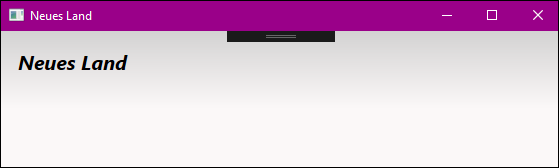
\includegraphics[scale=.75]{images/Wpf.png}
\end{center}
	\caption{Einfaches Wpf-Fenster}
	\label{fig:sample}
\end{figure}
Dennoch hat Wpf auch manche Nachteile:
\begin{itemize}
\item Der Computer muss eine moderne Grafikkarte haben sowie ein Betriebssystem haben, das jünger als Windows XP ist
\item Es kommt zu Leistungsproblemen, wenn mehrere Fenster im Einsatz sind und außerdem hat Wpf einen hohen RAM-Bedarf
\end{itemize}
\section{MVVM}
(Referenz Wiki MVVM) MVVM ist eine Abkürzung und steht für Model-View-ViewModel. Dies ist ein Muster, wie man Code designen kann und dient zur Trennung der Logik und Darstellung der Benutzerschnittstelle. Es ist speziell geeignet für Wpf. 
\begin{figure}[H]
\begin{center}
	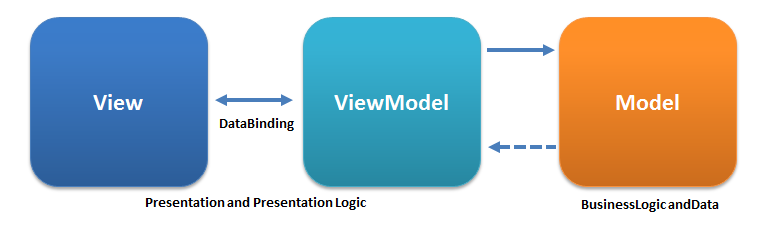
\includegraphics[scale=.75]{images/MVVMPattern.png}
\end{center}
	\caption{MVVM-Konzept}
	\label{fig:sample}
\end{figure}
(Foto von Wiki, Referenz Bucek Folien)
In der obenstehenden Grafik kann man leicht erkennen, wie MVVM funktioniert. Die View kommuniziert ausschließlich mit dem ViewModel und zwar über DataBindings. Das ViewModel beinhaltet die Logik und verändert gegebenenfalls das Model (Datenbank). 
\newline
Vorteile:
\begin{itemize}
\item Logik sowie Darstellung können unabhängig voneinander bearbeitet werden. Das hat wiederum den Vorteil, dass die Darstellung von Designern und die Logik von Entwicklern erstellt werden kann.
\item Durch die Trennung ergibt sich eine bessere Testbarkeit der Logik.
\end{itemize}
\section{MVVM-Light}
(Referenz dotnetcurry)
MVVM-Light ist ein Framework, welches dazu dient, die Implementierung des MVVM-Musters zu verringern. Neben MVVM-Light gibt es auch noch andere solcher Frameworks, wie zum Beispiel Prism. Zur Verwendung müssen die Packages MvvmLight (Version 5.3.0) und MvvmLightLibs (Version 5.3.0) über den NuGet-Package-Manager installiert werden. Beim Einbinden von MvvmLight werden zwei wesentliche Klassen erstellt
\begin{itemize}
\item MainViewModel: Das ViewModel der Hauptseite, abgeleitet von ViewModelBase.
\item ViewModelLocator: Beinhaltet statische Referenzen für alle anderen ViewModels. Außerdem bietet die Klasse einen einfachen IOC-Container an.
\end{itemize}
Alle ViewModels, die später erstellt werden, sollten von ViewModelBase abgeleitet werden. Damit hat der Programmierer die Möglichkeit die Methode RaisePropertyChanged zu verwenden. Diese ermöglicht dem ViewModel die View zu benachrichtigen, dass sich Daten verändert haben und somit kann die View die entsprechenden Daten aktualisieren. \newline
Hier werden die Daten der Kundenübersicht vom ViewModel aus aktualisiert.
\begin{lstlisting}
this.RaisePropertyChanged(() => this.CustomersView);
\end{lstlisting}
Im Gegenzug kann die View folgendermaßen auf eine Property im ViewModel binden:
\begin{lstlisting}
<ListView ItemsSource="{Binding CustomersView, Mode=TwoWay, UpdateSourceTrigger=PropertyChanged}">
\end{lstlisting}
MvvmLight enthält auch RelayCommands die zum Beispiel aufgerufen werden können, wenn ein Button gedrückt wird.
In der View kann man den Namen des ICommands angeben:
\begin{lstlisting}
<Button Command="{Binding DeleteFilter}">Filter zuruecksetzen</Button>
\end{lstlisting}
Und im ViewModel wird das gewünschte ICommand so initialisiert:
\begin{lstlisting}
DeleteFilter = new RelayCommand(DeleteF);
\end{lstlisting}
DeleteF ist dabei die Methode, die ausgeführt wird, sobald der Button gedrückt wird.
Ebenso gibt es die Möglichkeit andere Events der View zu abonnieren. Dazu müssen zusätzlich werden zwei Namespaces deklariert werden:
\begin{lstlisting}
xmlns:i="clr-namespace:System.Windows.Interactivity;
assembly=System.Windows.Interactivity"
xmlns:cmd="clr-namespace:GalaSoft.MvvmLight.Command;
assembly=GalaSoft.MvvmLight.Platform"
\end{lstlisting}
Im nachfolgenden Codeabschnitt wird das Event ''MouseDoubleClick'' vom ICommand ''OpenCustomer'' abonniert.
\begin{lstlisting}
<i:Interaction.Triggers>
                <i:EventTrigger EventName="MouseDoubleClick">
                    <cmd:EventToCommand Command="{Binding OpenCustomer}"></cmd:EventToCommand>
                </i:EventTrigger>
            </i:Interaction.Triggers>
\end{lstlisting}
\section{Microsoft Office Interop}
Um aus einem Programm Word-Dokumente zu erstellen, gibt es das Assembly Microsoft.Office.Interop.Word auf welches eine Referenz hinzugefügt wurde. Damit kann der Benutzer im Programm Word-Dokumente bearbeiten, oder Informationen herauslesen. Zur Nutzung benötigt der Computer allerdings eine gültige Microsoft Office Lizenz.  Außerdem lädt Interop das Word-Dokument im Hintergrund, wenn es bearbeitet wird, was den ganzen Vorgang etwas langsam macht.(Referenz Gembox)
Dennoch bietet sich der Gebrauch von Interop an, weil es die einfachste Variante ist, auf Word-Dokumente zuzugreifen.
Im folgenden Abschnitt wird erklärt wie aus einer Vorlage ein individuelles Word-Dokument erstellt werden kann.
\begin{lstlisting}
Application wordApp = new Application();
Document wordDoc = new Document();

Object oMissing = System.Reflection.Missing.Value;
wordDoc = wordApp.Documents.Add(ref oTemplatePath, ref oMissing, ref oMissing, ref oMissing);
foreach (Field myMergeField in wordDoc.Fields)
{
	Range rngFieldCode = myMergeField.Code;
	String fieldText = rngFieldCode.Text;

	//only mergefields should be edited
	if (fieldText.StartsWith(" MERGEFIELD"))
	{
		myMergeField.Select();
		wordApp.Selection.TypeText("Test");
	}
}
wordDoc.SaveAs(completePath);
wordDoc.Close();
wordApp.Quit();
\end{lstlisting}
Über den String ''oTemplatePath'' wird der Pfad des gewünschten Templates übergeben. Danach werden alle MergeFields der Vorlage (diese kann man beim Erstellen der Vorlage einfügen: Einfügen -\textgreater Schnellbaustein -\textgreater Mergefield) mit der Zeichenkette ''Test'' ersetzt. Im Endeffekt simuliert Interop einen Klick auf das Feld und mit der Methode TypeText(''Test'') wird der Text eingefügt. Zum Abschluss wird das Dokument unter einem angegeben Pfad abgespeichert (completePath) und die geöffnete Vorlage sowie die Applikation geschlossen.
\section{WPF-Toolkit}
Zur grafischen Darstellung der Statistiken wurde ebenfalls ein eigenes Assembly installiert:  System.Windows.Controls.DataVisualization.Toolkit (Version 4.0.0). Dieses Assembly kann einfach über den NuGetPackage-Manager heruntergeladen werden. Es ermöglicht die Veranschaulichung verschiedener Diagramme, wie zum Beispiel Linien-, Torten oder Balkendiagrammen. Zur Verwendung muss der Benutzer den Namespace in der View definieren.
\begin{lstlisting}
xmlns:toolkitCharting="clr-namespace:System.Windows.Controls.DataVisualization
.Charting;assembly=System.Windows.Controls.DataVisualization.Toolkit"
\end{lstlisting}
Im folgenden Code wird ein Liniendiagramm mit einer Linie erstellt:
\begin{lstlisting}
<toolkitCharting:Chart Title="{Binding Title}">
            <toolkitCharting:LineSeries Title="{Binding LineTitle}"  DependentValueBinding="{Binding Value}" IndependentValueBinding="{Binding Key}" ItemsSource="{Binding DataValues}"/>
</toolkitCharting:Chart>
\end{lstlisting}
In der Property ''Title'' wird der Titel des Diagramms übergeben und ''LineTitle'' beschriftet die Linie mit dem gewünschten Text. ''DataValues'' (Typ ''ObservableCollection\textless KeyValuePair\textless string, int\textgreater \textgreater'') beinhaltet die Daten, welche im Diagramm dargestellt werden sollen. DependentValueBinding=''\{Binding Value\}'' beschreibt, dass die abhängigen Werte des Diagramms jeweils vom Value bezogen werden. In DataValues ist das der int. 
\section{MessageBird}
(Referenz Website einbinden) MessageBird ist ein Unternehmen, welches einen Online-Dienst anbietet mit dem  Unternehmen oder auch einzelne Personen, kostenpflichtig SMS aus einem Programm aus zu versenden können. Dazu meldet sich der Benutzer auf der Website https://www.messagebird.com an und sucht sich das passende Angebot. Danach kann man sein Guthaben aufladen und bekommt im Gegenzug einen AccessKey, über den man Nachrichten versenden kann. Dabei kann jeder Benutzer von MessageBird mehrere AccessKeys haben, beispielsweise einen für Test-Nachrichten, die nicht wirklich versendet werden oder einen Key, mit dem dann echte SMS versendet werden. Für Nachrichten, die nach Österreich gesendet werden, muss der Benutzer 4,6 Cent zahlen. Sobald die SMS versendet wurde, wird der Betrag automatisch vom Guthaben des Benutzers abgezogen. Wenn das Guthaben aufgebraucht ist, versendet MessageBird keine SMS mehr und der Benutzer kann sein Guthaben gegebenenfalls wieder aufladen. Auf der Website hat man einen Überblick über die versendete SMS, verschiedene angelegte Nummern und vieles mehr. Im Code verwendet man MessageBird so:
\begin{lstlisting}
IProxyConfigurationInjector proxyConfigurationInjector = null; // for no web proxies, or web proxies not requiring authentication

Client client = Client.CreateDefault(AccessKey, proxyConfigurationInjector);

MessageBird.Objects.Message message = client.SendMessage("OptikAigner", this.Message, new[] { Convert.ToInt64(this.To) });
\end{lstlisting}

''AccessKey'' im zweiten Befehl ist der String, den man von der Website bekommt, über den abgerechnet wird. ''OptikAigner'' wird als Sendernamen angegeben.

\subsubsection{Andere Möglichkeiten}
Im Vergleich zum Versand von E-Mails, gibt es keine Möglichkeit kostenfrei und ohne Anbieter SMS zu versenden. Als Alternative hätte sich das Unternehmen ''Twilio'' angeboten, allerdings hätte dort eine SMS ca. 6 Cent gekostet und es wäre ein monatlicher Betrag zur Benutzung einer Nummer angefallen. Aus Kostengründen und aus Benutzerfreundlichkeit ist die Wahl des Anbieters auf MessageBird gefallen.